\section{Evidence status of headline claims}

\begin{table}[!htb]
\centering
\caption{Evidence status. \emph{Validated}: completed, with artifacts.
\emph{Qualified}: proxy validated, mechanism unresolved.
\emph{Provisional}: obtained earlier, not reproducible in the final
environment.}
\label{tab:evidence}
\small
\begin{tabular}{@{}p{0.62\linewidth}p{0.28\linewidth}@{}}
\toprule
\textbf{Claim} & \textbf{Status} \\
\midrule
Corrected JAB: 11 specimens, 396 fits; production $25.1\%$ WL & Validated \\
Expert supervision $26.9\%\to17.4\%$ (10/11 improve); no propagation to
  held-out regions & Validated \\
Coordinate-frame correction (\F{F7}) & Validated \\
Surface vs.\ skeleton dissociation ($0.45\times$ / $1.25\times$) & Validated \\
Regional-identity oracle $0.867\to0.937$ & Validated (synthetic) \\
PointNet: synthetic gain, real-scan transfer failure & Validated \\
W3 within-part gain; W5 deployment collapse & Validated (controlled) \\
SDF: real-scan instance-separation failure & Validated \\
Scale barrier & Qualified: proxy only \\
Corpus-scale (838-specimen) barrier validation & Not claimed \\
Genus-level permutation-null result & Provisional \\
Functional maps, OT, canonical fields & Future work \\
\bottomrule
\end{tabular}
\end{table}

\begin{table}[!htb]
\centering
\caption{Master experiment table: each investigation's hypothesis, evidence,
and the interpretation the evidence supports.}
\small
\begin{tabular}{@{}p{0.05\linewidth}p{0.23\linewidth}p{0.14\linewidth}p{0.18\linewidth}p{0.30\linewidth}@{}}
\toprule
\textbf{ID} & \textbf{Hypothesis tested} & \textbf{Data} & \textbf{Result} & \textbf{Interpretation} \\
\midrule
I1 & Error is a part-identity problem & Synthetic & Oracle $0.867\to0.937$ &
  Identity and within-region localisation are distinct; the latter dominates \\
I2 & Preprocessing dominates recovery & Real & Chamfer tie despite better
  topology & Mesh conditioning alone does not explain the failure \\
I3 & Surface score tracks anatomy & Real, expert & $0.45\times$ / $1.25\times$
  & Surface proximity and anatomical correctness can move in opposite
  directions \\
I4 & Initialisation explains failure uniformly & Synthetic & Distal
  recovers, coxa does not & Sensitivity is anatomically heterogeneous, not
  uniform \\
I5 & Objective directly observes skeleton position & Expert real &
  $25.1\%\to17.4\%$ with supervision, no propagation & Skeleton position is
  constrained only indirectly; supervision does not generalise spatially \\
I11 & Learned initialisation transfers to real data & Synth./real & Fails at
  the trained perturbation regime & Consistent with synthetic-to-real
  distribution mismatch \\
I14 & A local descriptor carries correspondence signal & Synthetic &
  $+16.4\%$ held-out improvement & Local learned signal exists beyond raw
  geometry \\
I15 & That signal deploys as dense correspondence & Synth./real & Coverage
  collapse ($28.1\%\to1.8\%$) & Pairwise retrieval accuracy does not imply
  globally consistent correspondence \\
\bottomrule
\end{tabular}
\end{table}

\begin{figure}[!htb]
\centering
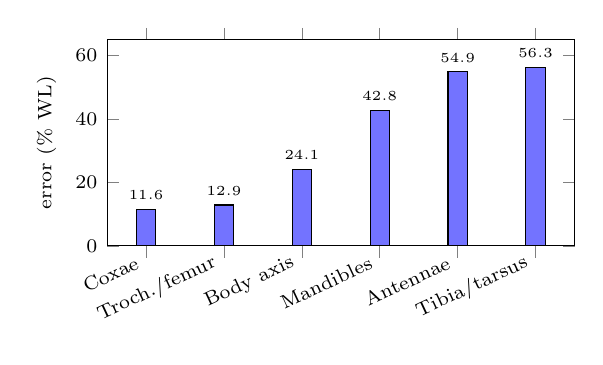
\begin{tikzpicture}
\begin{axis}[ybar,width=0.62\linewidth,height=4.2cm,bar width=7pt,ymin=0,ymax=65,
 symbolic x coords={Coxae,Troch./femur,Body axis,Mandibles,Antennae,Tibia/tarsus},
 xtick=data,x tick label style={rotate=25,anchor=east,font=\scriptsize},
 ylabel={error (\% WL)},ylabel style={font=\scriptsize},tick label style={font=\scriptsize},nodes near coords,
 every node near coord/.append style={font=\tiny}]
\addplot[fill=blue!55] coordinates {(Coxae,11.6)(Troch./femur,12.9)(Body axis,24.1)(Mandibles,42.8)(Antennae,54.9)(Tibia/tarsus,56.3)};
\end{axis}
\end{tikzpicture}
\hfill
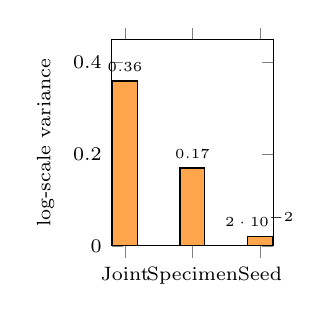
\begin{tikzpicture}
\begin{axis}[ybar,width=0.30\linewidth,height=4.2cm,bar width=9pt,ymin=0,ymax=0.45,
 symbolic x coords={Joint,Specimen,Seed},xtick=data,tick label style={font=\scriptsize},
 ylabel={log-scale variance},ylabel style={font=\scriptsize},nodes near coords,every node near coord/.append style={font=\tiny}]
\addplot[fill=orange!70] coordinates {(Joint,0.36)(Specimen,0.17)(Seed,0.02)};
\end{axis}
\end{tikzpicture}
\caption{Left: regional skeleton error on the corrected benchmark. Right:
variance decomposition; seed contributes almost nothing (\F{F8}).}
\label{fig:structured-error}
\end{figure}
